% !TeX root = ../main.tex
% -*- coding: utf-8 -*-


\chapter{基于梯度上升决策树的函数抽取重构推荐} 
本章针对最常见的软件重构操作--函数抽取重构操作进行研究。本章首先阐述了函数抽取对完善软件系统设
计、提高软件质量的重要作用,然后介绍了本章的研究动机以及相关工作。针对研究动机中的问题描述,本章提出
了基于数据驱动的函数抽取重构推荐模型,模型中融合了凝聚度、耦合度和复杂度的软件质量概念,并考虑了多种
程序元素。利用梯度上升决策树和逻辑斯特回归的融合模型,推荐函数抽取重构机会,从而帮助软件维护人员提高
维护效率。在实验部分,首先描述了实验设计,包括实验对象和评估方法。在对实验结果进行展示和分析后,讨论
了不同模型、数据集和特征对实验结果的影响,最后对本章进行小结。

\section{引言}
纠错性软件维护是保证软件正确性的重要手段,然而在纠错性维护后,虽然软件系统的正确性得以保障,但对软件
系统的修改可能会导致软件系统设计的偏离,使得软件质量降低。为了提高软件质量,通常需要后续进行完善性软
件维护。为了改进软件系统的设计,经常需要在不改变代码功能的前提下改变代码的结构,这种过程通常被称为软
件重构。软件重构作为一种重要的完善性软件维护手段,可以改善软件系统的设计、提高软件的易读性和可维护性
~\cite{fowler,mens:TSE04}。

大量的实践和研究表明,软件重构的作用主要有以下两种:(1)提高软件可维护性。当软件容易被理解时,软件
中的错误更容易被发现和修复~\cite{martin2009clean}。软件重构通过改进软件设计、重命名等方式,使得软件
设计更简单灵活、层次结构更清晰、代码更易被理解,从而减少代码维护的成本。(2)提高软件可扩展性。在软
件生命周期中,新的需求被不断添加,使得代码的复杂度越来越高,代码结构逐渐偏离原来的设计,从而导致了扩
展软件的难度越来越大。软件重构增加了程序设计的灵活性,通过改进软件设计,使得软件具备高凝聚、低耦合和
复杂度低等特点,将复杂代码变简单,从而提高代码的可扩展性。

软件重构机会推荐作为一种自动化软件维护的手段,一直是研究者们较为关注的课题。软件重构机会推荐指的是推
荐软件系统中能够改善软件系统设计、提高软件质量但尚未被实施的重构机会
~\cite{fokaefs:icse11,higo:JSME,Liu:IEEE-TSE:12,Tourwe:CSMR03,Tsantalis:2011}。软件重构机会推荐可以
提高软件理解和维护的效率。Murphy-Hill等人~\cite{Murphy-Hill:ICSE09}对99个使用Eclipse集成开发工具的
Java开发人员进行了一个调研,发现函数抽取重构(Extract Method,简称EM)是最常用的软件重构类型之
一。函数抽取重构是在改变函数功能的前提下重新组织函数,把其中部分代码片段抽取出来并组成新的函数代替原
来的代码片段被调用。函数抽取重构的原因较为复杂,包括代码重用、长函数分解、重命名内部函数等11中主要原
因~\cite{silva2016we}。虽然函数抽取重构的原因较为复杂,但通常被抽取的代码段执行一个具体的、明确的功
能。正因为此,函数抽取重构通常可以改善软件系统的设计,提高易读性和可维护性。

虽然函数抽取重构被认为是最常被使用的软件重构类型之一~\cite{Murphy-Hill:ICSE09},但根据Kim等人的调研
报告,58.3\%的被调研者手动进行所有的函数抽取重构操作~\cite{Kim:FSE12}。同样,根据JDeodorant(著名的
重构机会推荐工具)的使用统计,函数抽取重构占所有被执行的重构操作的25\%,然而只有4.4\%的函数抽取重构
时通过Eclipse集成开发环境执行~\cite{Negara:ECOOP13,Murphy-Hill:ICSE09}。研究表明,开发和设计用于自动
推荐函数抽取重构机会的推荐系统可以在集成开发环境中发挥重要的作用~\cite{Tsantalis:2011}。

为了帮助软件维护人员提高软件重构的效率,研究者们开发了针对函数抽取重构的推荐工具。目前主流的函数抽取
重构机会推荐工具有:Fokaefs等人设计的JDeodorant~\cite{fokaefs:icse11},该工具基于程序切片技术选择可
以被提取到一个新函数的相关代码;Silva等人开发的JExtract~\cite{silva:CoRR15},根据最大化凝聚度和最小
化耦合度的软件设计原则,设计了一个排序函数为候选函数抽取重构机会打分,抽取相对独立的、与剩余代码依赖
性较小的代码片段来组成新函数~\cite{silva:ICPC14};类似的,Charalampidou等人提出了
SEMI~\cite{charalampidou2016identifying},提取在距离在一定范围内的相关代码片段,并根据是否存在共同变
量来判断代码语句的相关性,最后针对所有的候选函数抽取重构机会,根据软件度量$LCOM_2$进行排序推荐。

尽管大多数函数抽取重构推荐技术旨在推荐改善软件设计的重构机会,但是由于软件设计的优劣和软件质量的好坏
很难通过具体的公式进行定义,以提高软件质量为目标的函数抽取重构推荐技术,大多通过特定的软件度量或
自定义函数对重构机会进行推荐,忽略了其它跟函数抽取重构相关的因素。然而函数抽取重构的原因较为复杂多
样,因此目前这些推荐方法的效果不甚理想。例如,软件度量LCOM(Lack of Cohesive Metric),只考虑了
具有共同变量的语句的个数作为凝聚力的象征,而其它与函数抽取和程序功能相关的因素并没有被考虑进去。

本章提出基于机器学习的函数抽取重构机会推荐模型,通过提取一组结构特征和一组功能特征来对候选函数抽取重
构机会进行表示。具体来说,在特征提取算法中,提取了一组与函数和候选代码片段的复杂度相关的结构特征,以
及一组与凝聚度和耦合度相关的功能特征。与传统的软件度量不同,该模型将软件质量相关的特征用一系列程
序元素来表示,包括与代码功能相关的变量使用、函数调用和包等。通过融合多种软件质量概念和程序元素,将函
数抽取重构机会表示为可供学习的特征序列。通过从开源软件仓库中挖掘真实存在的函数抽取重构实例,模型可以
从中学习到关于函数抽取重构的概率模型。给定一个新的函数体,该模型生成的候选函数抽取重构机会,并为每个
合法的重构机会分配一个概率,表示该重构机会为使用者所采纳的可能性,并按照概率由高至低进行推荐。

本章具有以下贡献:

(1)提出了一个关于函数抽取重构的概率模型,通过学习从开源软件仓库中挖掘到的重构实例,模拟了软件维护
人员进行软件重构的过程,并考虑了函数抽取重构原因的多样性。

(2)提出了关于结构特征和功能特征的特征提取算法,融合了凝聚度、耦合度、复杂度的软件质量概念,并考虑
了多种程序元素。

(2)设计并开发了一个基于Eclipse的插件,为给定Java函数生成函数抽取重构机会,并为每个合法的候选重构机会
分配一个概率,按照概率由高至低推荐给集成开发环境使用者。

(3)在开源程序上与主流函数抽取重构推荐工具的对比实验证明了方法的有效性,能够更准确地推荐函数抽取重
构机会,为软件维护人员提高维护效率。

\section{研究动机与相关工作}
与纠错性软件件维护不同,完善性软件维护通常没有统一的、明确的标准来量化维护的效果。由于完善性软件维
护,尤其是软件重构的主要目的是改善软件系统的设计和提高软件质量,因此当前主流的面向函数抽取重构机会的
推荐技术采用软价质量度量作为评判重构机会的方法。然而,考虑到函数抽取重构的原因的多样性
~\cite{silva2016we}和软件度量的片面性,根据软件度量进行函数抽取重构机会推荐的效果往往不甚理想。

\subsection{研究动机}
图~\ref{before-code}为来自AsyncHttpClient库的示例代码

\begin{figure}
\centering
\subfigure[2个缺陷]{\label{fig:temp_nuh}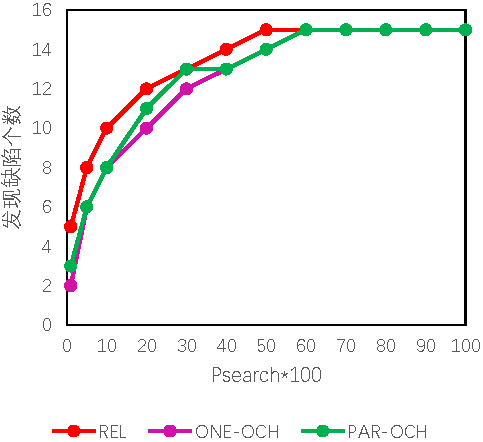
\includegraphics[width=0.49\linewidth]{fault2.pdf}}
\vskip\baselineskip
\subfigure[3个缺陷]{\label{fig:temp_synpuf}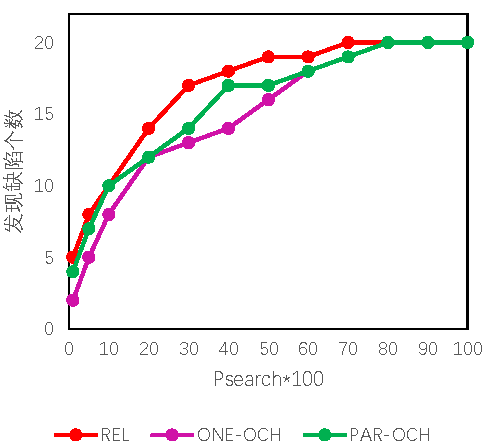
\includegraphics[width=0.49\linewidth]{fault3.pdf}}
\vskip\baselineskip
\subfigure[4个缺陷]{\label{fig:temp_nuh}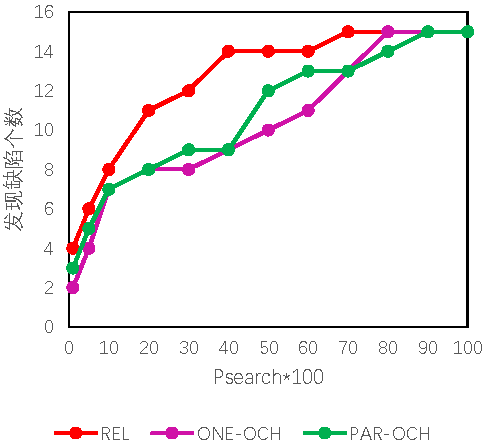
\includegraphics[width=0.49\linewidth]{fault4.pdf}}
\caption{基于覆盖分析的多缺陷定位方法的实验结果}
\label{fig:multi}
\end{figure}


\iffalse

\begin{figure}\label{before-code}
  \centering
  \subfigure[函数抽取重构前函数]{
    \begin{lstlisting}[columns=fullflexible,label={lst:label}]
   public String calculateSignature(...) {
          String baseUrl = baseUrl(uri);
          String encodedParams = encodedParams(oauthTimestamp...queryParams);
          StringBuilder sb = StringUtils.stringBuilder();
          sb.append(method);
          sb.append('&');
          Utf8UrlEncoder.encodeAndAppendQueryElement(sb, baseUrl);
          sb.append('&');
          Utf8UrlEncoder.encodeAndAppendQueryElement(sb, encodedParams);
          ByteBuffer rawBase = StringUtils.charSequence2ByteBuffer(sb, UTF_8);
          byte[] rawSignature = mac.digest(rawBase);
          return Base64.encode(rawSignature);
      }
    \end{lstlisting}
  }
\end{figure}
\fi

\begin{figure}\label{after-code}
  \centering
    \begin{lstlisting}[columns=fullflexible,label={lst:label}]
   public String calculateSignature(...) {
          String sb = encodeParameter(uri...method);
          ByteBuffer rawBase = StringUtils.charSequence2ByteBuffer(sb, UTF_8);
          byte[] rawSignature = mac.digest(rawBase);
          return Base64.encode(rawSignature);
      }
    \end{lstlisting}
    \caption{函数抽取重构后函数}
\end{figure}

\begin{figure}\label{after-code}
  \centering
    \begin{lstlisting}[columns=fullflexible,label={lst:label}]
   public String encodeParameter(...) {
          String baseUrl = baseUrl(uri);
          String encodedParams = encodedParams(oauthTimestamp...queryParams);
          StringBuilder sb = StringUtils.stringBuilder();
          sb.append(method);
          sb.append('&');
          Utf8UrlEncoder.encodeAndAppendQueryElement(sb, baseUrl);
          sb.append('&');
          Utf8UrlEncoder.encodeAndAppendQueryElement(sb, encodedParams);
          return sb;
      }
    \end{lstlisting}
    \caption{新函数}
\end{figure}


\begin{table}[!t]
  \renewcommand{\arraystretch}{1.3}
  % if using array.sty, it might be a good idea to tweak the value of
  % \extrarowheight as needed to properly center the text within the cells
  \caption{Method-level Metrics of the Candidates in the Example}
  \label{example_metrics}
  \centering
  %% Some packages, such as MDW tools, offer better commands for making tables
  %% than the plain LaTeX2e tabular which is used here.
  %\begin{tabular}{|p{0.1cm}p{0.55cm}p{0.6cm}p{0.6cm}p{0.8cm}||p{0.1cm}p{0.55cm}p{0.6cm}p{0.6cm}p{0.8cm}|}
  %\begin{tabular}{|p{0.1cm}p{0.55cm}p{0.6cm}p{0.6cm}p{0.8cm}||p{0.1cm}p{0.55cm}p{0.6cm}p{0.6cm}p{0.8cm}|}
  \begin{tabular}{ccccc|ccccc}
  \toprule No. &Cand &M1 &M2 &M3 &No. &Cand &M1 &M2 &M3\\ \midrule 1 &2-7 &8 &0 &6
   &9 &3-10 &6 &0 &6\\
   2 &2-8 &10 &0 &6 &10 &3-11 &13 &0 &6\\
   3 &\textbf{2-9} &11 &0 &6 &11 &3-12 &21 &0 &6\\
   4 &2-10 &13 &0 &6 &12 &4-9 &0 &0 &3\\
   5 &2-11 &28 &3 &6 &13 &4-10 &0 &0 &3\\
   6 &2-12 &36 &10 &6 &14 &5-7 &0 &0 &3\\
   7 &3-8 &4 &0 &6 &15 &5-8 &0 &0 &3\\
   8 &3-9 &5 &0 &6 &16 &5-9 &0 &0 &4\\
   \bottomrule
  \end{tabular}
  \end{table}
  




\subsection{相关工作}
\section{研究方法}
\subsection{特征提取算法}

\begin{figure}[bth]
  {\scriptsize
	\begin{center}
	  \begin{algorithmic} [1]
%                        \Procedure{feature\_extract}{$m,b,P$}
			\REQUIRE  : The input method \textit{m}, the selected block
			\textit{b} and the set of program elements \textit{P}
			\ENSURE The feature vector % \textit{feature\_extract(\textit{m},\textit{b},\textit{P})
			\STATE $S_M  \leftarrow getStmts(m)$
			\STATE $S_B  \leftarrow getStmts(b)$
			\FOR{$p$ in $P$}
				\STATE $E \leftarrow getElmts(b, p)$
				\FOR{$e$ in $E$}			
					\STATE $freq_M \leftarrow getFreq(m, e)$
					\STATE $freq_B \leftarrow getFreq(b, e)$
					\STATE $ratio_e \leftarrow freq_B / freq_M$
				\ENDFOR
				\STATE $idx \leftarrow \textit{idxOfMax}(ratio_E)$
				\STATE $cp \leftarrow ratio_{idx}$
				\STATE $loc \leftarrow getLOC(b)$				
				\STATE $count \leftarrow 0$				
				\FOR{$s$ in $S_B$}
					\IF{$E_{idx}$ in $getElmts(s)$}
						\STATE $count \leftarrow count + 1$
					\ENDIF
				\ENDFOR
				\STATE $ch \leftarrow count / loc$ 
				\STATE $setFeature(p, cp, ch)$
			        \ENDFOR
%                                \EndProcedure
		\end{algorithmic}
	\end{center}
        }
	\caption{Extraction Algorithm of Metric-related Features}
	\label{feature_algorithm}
\end{figure}
\subsection{梯度上升决策树模型}
\subsection{候选函数抽取重构操作生成}
\section{实验设计}
\subsection{实验对象}
\begin{table}[!t]
  \renewcommand{\arraystretch}{1.3}
  % if using array.sty, it might be a good idea to tweak the value of
  % \extrarowheight as needed to properly center the text within the cells
  \caption{Statistics of Subject Systems}
  \label{benchmark}
  \centering
  \begin{tabular}{ccc}
  \toprule 
  Projects &Methods &Refactor.\\ \midrule
  JHotDraw &56 &56 \\ 
  Junit &25 &25 \\ 
  MyWebMarket &23 &35 \\ 
  SelfPlanner &12 &13 \\ 
  Wikidev &14 &26 \\ \midrule
  Total &130 &155 \\ 
  \bottomrule
  \end{tabular}
  \end{table}

\subsection{实验方法}

\subsection{评估指标}

\section{实验结果与分析}

\begin{table}[!t]
  \renewcommand{\arraystretch}{1.3}
  % if using array.sty, it might be a good idea to tweak the value of
  % \extrarowheight as needed to properly center the text within the cells
  \caption{Accuracy of Different Approaches}
  \label{accuracy}
  \centering
  \begin{tabular}{cc|ccc}
  \toprule
   Tools &Tolerance &Precision &Recall &F-measure\\ 
  \hline
  \multirow{4}{*}{GEMS$^{GB}$}&$1\%$ &\bf{22.5\%} &\bf{54.2\%} &\bf{31.8\%} \\ 
  &$2\%$ &\bf{28.5\%} &\bf{59.8\%} &\bf{38.6\%} \\ 
  &$3\%$ &\bf{34.3\%} &\bf{62.6\%} &\bf{44.3\%} \\ 
  \hline
  \multirow{4}{*}{JExtract}&$1\%$ &12.6\% &52.2\% &20.4\% \\ 
  &$2\%$ &13.1\% &\bf{59.3\%} &21.5\% \\ 
  &$3\%$ &15.0\% &61.9\% &24.2\% \\ 
  \hline
  \multirow{4}{*}{SEMI}&$1\%$ &12.9\% &38.0\% &19.2\% \\ 
  &$2\%$ &14.6\% &47.0\% &22.3\% \\ 
  &$3\%$ &18.8\% &55.5\% &28.1\% \\ 
  \hline
  \multirow{4}{*}{JDeodorant}&$1\%$ &17.4\% &14.8\% &16.0\% \\
  &$2\%$ &21.1\% &18.4\% &19.7\% \\ 
  &$3\%$ &28.0\% &23.8\% &25.7\% \\ 
  \bottomrule
  \end{tabular}
  \end{table}

\begin{table}[!t]
  \renewcommand{\arraystretch}{1.3}
  % if using array.sty, it might be a good idea to tweak the value of
  % \extrarowheight as needed to properly center the text within the cells
  \caption{Accuracy in Long methods}
  \label{long_methods}
  \centering
  \begin{tabular}{cc|ccc}
  \toprule
   Tools &Tolerance &Precision &Recall &F-measure\\ 
  \hline
  \multirow{4}{*}{GEMS$^{GB}$}&$1\%$ &13.3\% &31.9\% &18.8\% \\ 
  &$2\%$ &\bf{17.4\%} &\bf{41.5\%} &\bf{24.5\%} \\ 
  &$3\%$ &\bf{25.3\%} &\bf{46.2\%} &\bf{32.7\%} \\ 
  \hline
  \multirow{4}{*}{JExtract}&$1\%$ &6.6\% &16.1\% &9.4\% \\ 
  &$2\%$ &8.0\% &19.3\% &11.3\% \\ 
  &$3\%$ &8.0\% &19.3\% &11.3\% \\ 
  \hline
  \multirow{4}{*}{SEMI}&$1\%$ &\bf{16.4\%} &\bf{38.7\%} &\bf{23.0\%} \\ 
  &$2\%$ &\bf{17.9\%} &\bf{41.9\%} &\bf{25.0\%} \\ 
  &$3\%$ &19.1\% &45.1\% &26.9\% \\ 
  \hline
  \multirow{4}{*}{JDeodorant}&$1\%$ &12.0\% &9.6\% &10.7\% \\
  &$2\%$ &14.3\% &12.9\% &13.5\% \\ 
  &$3\%$ &16.0\% &12.9\% &14.2\% \\ 
  \bottomrule
  \end{tabular}
  \end{table}

\section{讨论}

\section{本章小结}
虽然已经开发完成的Eclipse插件是面向Java语言的,但只需要改变特征向量的生成方式,,本章方法可同样适用
于其它语言。